%#######################################################################

In this section, we discuss distance correlation, their benefits
and their mathematical properties. Distance correlations first appeared
in  \cite{szekely2007measuring} but has seen made multiple appearances
in other papers stating various extensions and applications. The two
followup papers that contain a thorough survey of these extensions are
in \cite{szekely2013energy} and \cite{sejdinovic2013equivalence}.

As we will see, the distance correlation is a non-linear measurement of
the dependency between two distributions, and it equals zero if and only
if the two distributions are independent of one another. This
measurement will be used to determine which spatially-adjacent voxels
are related and serves as the statistical foundation of our parcellation
procedures. While many works have gone ahead to use distance correlation
to test the null hypothesis that two distributions are independent, we
simply use the distance correlation as a statistical guide to aid our
graph-based algorithms generate a reasonable parcellation.

\section{Benefits of Distance Correlation}

To measure dependence, statisticians have traditionally used the Pearson
correlation coefficient, in addition to the rank-based Kendall tau and
Spearman rho. These statistics work well when the underlying
relationship between the two random variables is linear, in the case of
Pearson, or can be linear after a monotonic transformation, in the case
of Kendall and Spearman. Due to their restrictions, these correlation
coefficients will fail to capture many kinds of dependency
relationships. The figure below illustrates several instances of pairs
of random variables whose depencency structure is not detected by the
three correlation coefficients.

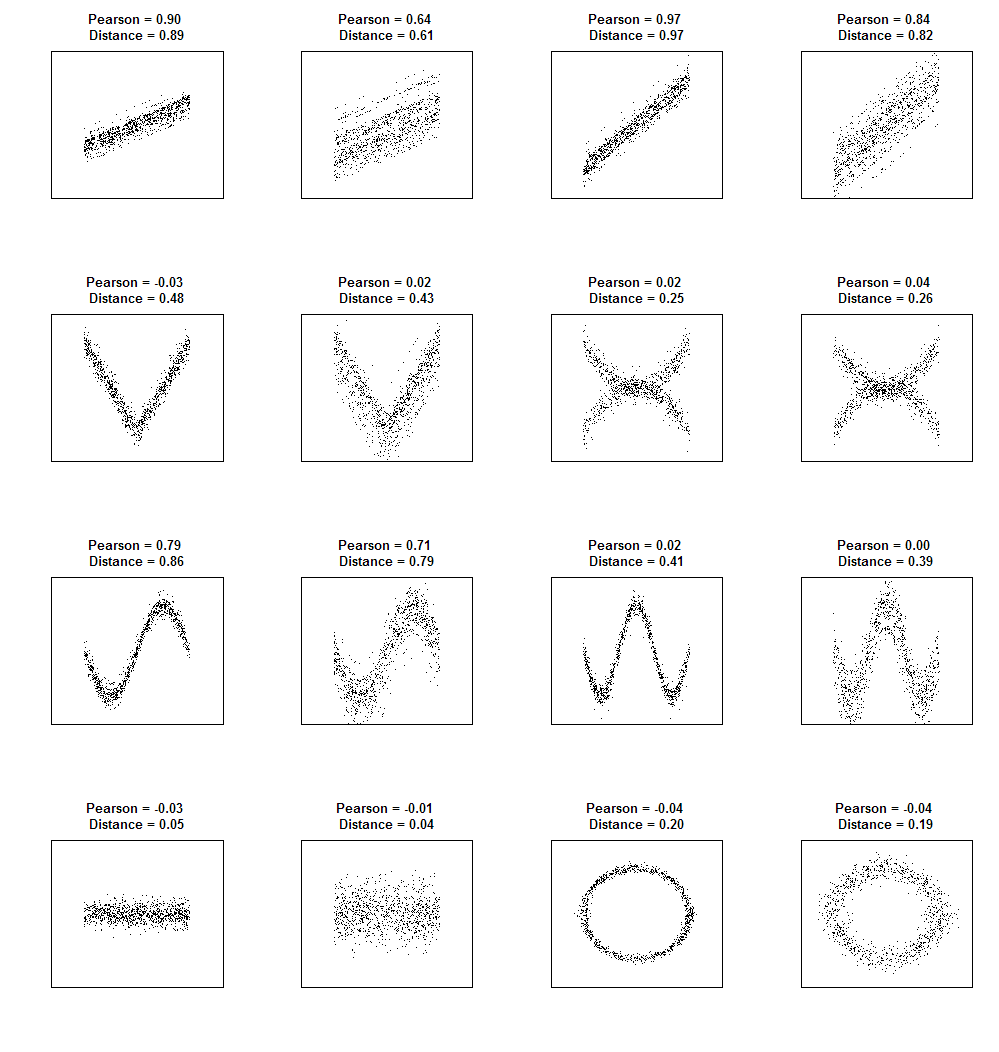
\includegraphics[scale = 0.8]{figs/1_nonlinear_depend.png}

Non-linear dependency relationships also exist in the ABIDE 50002 fMRI
data. The scatterplots below show time samples of spatially adjacent
voxels. These instances were found by searching for the maximum
difference in rank of energy distance correlation and the coefficient
of determination, or Pearson squared.

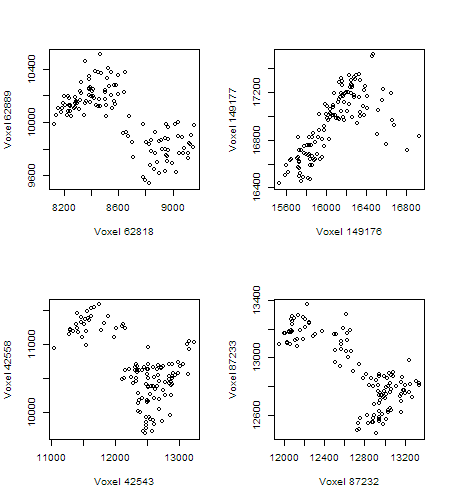
\includegraphics[scale = 0.7]{figs/1_nonlinear_ABIDE_50002.png}

\section{Distance Covariance}

We first discuss the definition of distance covariance, from which the
definition of distance correlation will naturally follow. We first start
with the population quantity where $\mathcal{V}^2(X,Y)$ represents the
population distance covariance between two distributions, one over the
random variable $X$ in a $p$-dimensional space and the other over $Y$ in
a $q$-dimensional space. In our application, $p=q$. Let $\varphi_X$
denote the characteristic function associated with the density of $X$.
For some positive weight function
$w : \R^p \times \R^q \mapsto [0, \infty)$ define the norm
$\|\cdot\|_w : \{\gamma : \R^p \times \R^q \mapsto \mathbb{C}\}
               \mapsto [0, \infty)$ as
$$ \| \gamma \|_w^2 = \int_{\R^{p+q}} | \gamma(s,t) |^2 w(s,t) ds dt. $$

In the case where the subscript $w$ is omitted, it is implied that
$w = 1$, the constant function taking value one. Hence $\| \cdot \|^2$
is the typical definition of the $\ell_2$ (Euclidean) norm squared.

\begin{definition}[Distance covariance] 
Let $X$ and $Y$ be two $d$-dimensional random
vectors with $\Expect\|X\| + \Expect\|Y\| < \infty$. Their distance
covariance is
\begin{align*}
\mathcal{V}^2 (X,Y)
&= \| \varphi_{X,Y}(s,t) - \varphi_X(s)\varphi_Y(t) \|_w^2 \\
&= \int_{\R^{p+q}} \dfrac{|\varphi_{X,Y}(s,t) -
                           \varphi_X(s)\varphi_Y(t)|^2}
                         {\|s\|^{1+p} \|t\|^{1+q}} ds dt
\end{align*}
where $w(s,t) = \dfrac{1}{\|s\|^{1+p} \|t\|^{1+q}}$.
\end{definition}

It is clear that $\mathcal{V}^2(X,Y) = 0$ if and only if  $X \indep Y$.
To explicitly see why this is called a distance \emph{covariance}, we
notice that the definition of $\mathcal{V}^2(X,Y)$ can be rewritten in
terms of covariances. Let $X, X', X''$ be three independent copies of
the same random variable but drawn from the same distribution.

\begin{prop}[\cite{szekely2003statistics} (Theorem 1)] \label{prop:cov}
\begin{align*}
\mathcal{V}^2 (X,Y)
&= \Expect[\|X - X'\| \|Y - Y'\|]
 + \Expect[\|X - X'\|] \Expect[\|Y - Y'\|]
 - 2 \Expect[ \|X - X'\| \|Y - Y''\| ] \\
&= \Cov( \|X - X'\|, \|Y - Y'\| ) - 2 \Cov (\|X - X'\|, \|Y - Y''\| ) 
\end{align*}
\end{prop}

With a slight overload of notation, we define the distance variance to be
the distance covariance between the same variable. 
\begin{definition}
[Distance variance]
$$ \mathcal{V}^2 (X) = \mathcal{V}^2 (X,X) $$
\end{definition}

Using the standard relationship between covariance and correlation, we 
define the distance correlation as such. It is clear from the definition
that this quantity is bounded between $\pm 1$, much like the Pearson
correlation.

\begin{definition}
[Distance correlation]
$$ \mathcal{R}^2 (X,Y) = \dfrac{\mathcal{V}^2(X,Y)}
                               {\mathcal{V}(X) \mathcal{V}(Y)} $$
\end{definition}

The above definitions all hold for the population quantities, but now
we are interested in estimating them. While the population distance
covariance (and the population distance correlation) are equal to 0 if
and only if the two distributions are independent, we hope to estimate a
sample distance correlation which is close but not necessarily 0 when
the two distributions are independent.

For independent, identically-distributed sample $\{(X_i, Y_i)\}_{i=1}^n$,
let $\widehat{\varphi}_X (t) = \frac{1}{n} \sum_{i=1}^n \exp(i t^T X_i)$ 
be the empirical characteristic function for $X$ and likewise for $Y$. An
estimate of $\mathcal{V}^2(X,Y)$ replaces the unknown characteristic
functions with the empirical characteristic functions. Thanks to
Proposition \ref{prop:cov}, we will simply replace the expectations by
the same averages.

\begin{definition}[Sample Distance Covariance]
$$ \widehat{\mathcal{V}}^2 (X,Y) \equiv
\| \widehat{\varphi}_{X,Y}(s,t) -
            \widehat{\varphi}(s) \widehat{\varphi}_Y(t) \|_w^2
  = S_1 + S_2 - 2 S_3 $$
where 
\begin{align*}
S_1 &= \frac{1}{n^2} \sum_{k=1}^n \sum_{l=1}^n \|X_k - X_l\| \|Y_k - Y_l\| \\
S_2 &= \left( \frac{1}{n^2} \sum_{k=1}^n \sum_{l=1}^n \|X_k - X_l\| \right) \frac{1}{n^2} \sum_{k=1}^n \sum_{l=1}^n \|Y_k - Y_l\| \\
S_3 &= \frac{1}{n^3} \sum_{k=1}^n \sum_{l=1}^n \sum_{m=1}^n \|X_k - X_l\| \|Y_k - Y_m\|
\end{align*}
Alternatively, we can let $A, B \in \R^{n \times n}$ such that
$A_{kl} = \|X_k - X_l\|$ and $B_{kl} = \|Y_k - Y_l\|$ ($A$ and $B$ are
symmetric elementwise nonnegative). Let
$\overline{X} = \frac{1}{n^2} \sum_{k,l = 1}^n X_{kl}$. Then
$$ \widehat{\mathcal{V}}^2 (X,Y)
 = \overline{A \circ B} + \overline{A} \cdot \overline{B} - \frac{2}{n}
   (\overline{A B}) $$
where $\circ$ means element-wise multiplication.
\end{definition}


Estimates of distance variance and distance correlation are defined
analogously.

\section{Statistical Review}
We now review some key properties that relate the sample distance
covariance to the population distance covariance that helps give
insight. We simply state the theorems and refer to the papers for
interested readers.

First, we relate the distance correlation to Pearson correlation.

\begin{definition} [$\alpha$-distance covariance] 
For $0 < \alpha < 2$
$$ \mathcal{V}_\alpha^2 (X,Y)
 = \frac{1}{C(p,\alpha) C(q,\alpha)}
   \int_{\R^{p+q}} \frac{|\varphi_{X,Y}(s,t) -
                          \varphi_X(s) \varphi_Y(t)|^2}
                        {\|s\|^{\alpha + p} \|t\|^{\alpha + q}} ds dt $$
\end{definition}

\begin{prop}[\cite{szekely2013energy} (Section 7.2)]
If $\Expect[\|X\|^\alpha] + \Expect[\|Y\|^\alpha] < \infty$ then
$$ \mathcal{V}_\alpha^2 (X,Y) = \Expect[ \|X - X'\|^\alpha \|Y - Y'\|^\alpha ] + \Expect \|X - X'\|^\alpha \Expect \|Y - Y'\|^\alpha - 2 \Expect[ \|X - X'\|^\alpha \|Y - Y''\|^\alpha ]$$

In particular, if $\alpha = 2$, $p = q = 1$, the distance correlation is 
the absolute value of Pearson's correlation coefficient.
\end{prop}

Next, we show statement ensuring consistency under the existence of the
first moments.

\begin{prop}[\cite{szekely2007measuring} (Corollary 1)]
If $\mathbb{E}(\|X\| +\|Y\|)< \infty$, then almost surely
\[
\lim_{n\rightarrow\infty}\widehat{\mathcal{R}}(X,Y) = \mathcal{R}(X,Y)
\]
\end{prop}

While we did not find a theorem explicitly stating the rate of 
convergence, the above theorem gives us satisfaction that if
$\mathcal{V}(X,Y)=0$ (meaning $X$ and $Y$ are independent), then as long 
as we have enough samples, $\widehat{\mathcal{V}}(X,Y) $ will approach
0. In our case, $n$ refers to the number of time samples which
typically range from $n=100$ to $n=200$.

We next show the asymptotic distribution of the sample distance
covariance under independence of $X$ and $Y$. While this is not used in
our work (as we do not apply the hypothesis test), this can inspire
future work where instead of computing the sample energy statistics
$\widehat{\mathcal{V}}(X,Y)$, we compute the $p$-value
under the null hypothesis $H_0: X \indep Y$.

To formulate the asymptotic distribution, we need additional notation.
Let $Q$ be a random variable where
\[ Q \overset{D}{=} \sum_{j=1}^{\infty}\lambda_j Z^2_j, \]
where $Z_j$ are independent, standard normal random variables and
$\{\lambda_j\}$'s are nonnegative constants dependent on the
characteristic functions on the joint distribution $(X,Y)$ such that
$\mathbb{E}[Q] = 1$. Here, we put the superscript $D$ to denote equality 
in distribution.

\begin{prop}[\cite{szekely2007measuring} (Corollary 2)]
If $\mathbb{E}(\|X\| +\|Y\|)< \infty$, then
\begin{itemize}
\item If $X$ and $Y$ are independent, then $n\widehat{\mathcal{V}}^2/S_2 \overset{D}{\rightarrow} Q$.
\item If $X$ and $Y$ are dependent, then $n\widehat{\mathcal{V}}^2/S_2 \overset{P}{\rightarrow} \infty$.
\end{itemize}
\end{prop}

Here, the superscript $D$ and $P$ denote convergence in distribution and
probability as $n$ goes to infinity. More explicit asymptotic
distributions are given in \cite{szekely2013energy} when $X$ and $Y$ are
Gaussian, but in general, bootstrapping procedures can be used to test
this hypothesis. Similar procedures can be derived on the distance
correlation.

In all our computations throughout our thesis, we use the \texttt{dcor}
function in the \texttt{energy} package to compute the distance
correlation efficiently.
